%!TEX program = xelatex
\documentclass[a4paper,12pt]{ctexart}

%==================== 1. 宏包引入 ====================
\usepackage{geometry}       % 页面设置
\usepackage{graphicx}       % 图片支持
\usepackage{amsmath, amssymb, amsfonts, amsthm} % 数学公式与符号
\usepackage{booktabs}       % 三线表(论文标准表格)
\usepackage{caption}        % 图表标题设置
\usepackage{float}          % 图片浮动位置控制
\usepackage{titlesec}       % 标题格式精细控制
\usepackage{fontspec}       % 字体设置
\usepackage{setspace}       % 行距设置
\usepackage{hyperref}       % 超链接与引用跳转
\usepackage{algorithm}      % 算法伪代码
\usepackage{algorithmic}    % 算法内容
\usepackage{multirow}       % 表格多行合并
\usepackage{subfig}         % 子图支持
\usepackage{cite}           % 参考文献引用优化

%==================== 2. 页面与字体设置 (严格匹配Word模板) ====================

% --- 页边距 ---
\geometry{left=3.17cm, right=3.17cm, top=2.54cm, bottom=2.54cm}

% --- 字体设置 ---
% 这里的设置适配 Windows 环境。如果编译报错,请注释掉下面三行,使用默认字体。
\setmainfont{Times New Roman}
\setCJKmainfont[BoldFont=SimHei, ItalicFont=KaiTi]{SimSun} % 正文宋体,粗体对应黑体
\setmonofont{Courier New}

% --- 字号定义 (对应 Word 字号) ---
\newcommand{\sanhao}{\fontsize{16pt}{\baselineskip}\selectfont}      % 三号
\newcommand{\xiaosan}{\fontsize{15pt}{\baselineskip}\selectfont}     % 小三
\newcommand{\sihao}{\fontsize{14pt}{\baselineskip}\selectfont}       % 四号 (14pt)
\newcommand{\xiaosi}{\fontsize{12pt}{\baselineskip}\selectfont}      % 小四 (12pt, 正文标准)
\newcommand{\wuhao}{\fontsize{10.5pt}{\baselineskip}\selectfont}     % 五号 (10.5pt)
\newcommand{\xiaowu}{\fontsize{9pt}{\baselineskip}\selectfont}       % 小五 (9pt)

% --- 行距 ---
\onehalfspacing % 1.5倍行距,视觉上接近Word的单倍行距效果

%==================== 3. 标题格式设置 ====================

% 一级标题:三号黑体,居中,段前段后间距优化
\titleformat{\section}{\centering\heiti\sanhao}{\thesection}{1em}{}
\titlespacing*{\section}{0pt}{1.5ex plus .2ex minus .2ex}{1ex plus .2ex}

% 二级标题:四号黑体,左对齐
\titleformat{\subsection}{\heiti\sihao}{\thesubsection}{1em}{}
\titlespacing*{\subsection}{0pt}{1.2ex plus .2ex minus .2ex}{0.8ex plus .2ex}

% 三级标题:小四号黑体,左对齐
\titleformat{\subsubsection}{\heiti\xiaosi}{\thesubsubsection}{1em}{}
\titlespacing*{\subsubsection}{0pt}{1ex plus .2ex minus .2ex}{0.5ex plus .2ex}

% --- 图表标题格式 ---
\DeclareCaptionFont{mysize}{\wuhao} % 使用五号字
\captionsetup[figure]{font=mysize, name=图, labelsep=quad} % 图注格式
\captionsetup[table]{font=mysize, name=表, labelsep=quad}  % 表注格式

%==================== 4. 论文正文开始 ====================
\begin{document}

%---------- 封面/标题区 ----------
\begin{center}
    \vspace*{1em}
    % 论文题目:三号黑体加粗
    {\heiti\sanhao \textbf{基于谱归一化的深度强化学习可塑性丢失改进研究}}\\ 
    \vspace{2em} 
    
    % 作者信息:四号宋体
    {\songti\sihao 
    电子与信息工程学院 \quad 宋凯\\ 
    学号:2023280466 
    }
    \vspace{2em}
\end{center}

%---------- 摘要区 ----------
\begin{center}
    \begin{minipage}{0.95\textwidth} % 摘要宽度略窄于正文,显美观
        % 摘要标题:小四黑体
        {\heiti\xiaosi \textbf{【摘要】}} 
        % 摘要正文:五号宋体
        {\songti\wuhao 
        深度强化学习(Deep RL)在处理非平稳环境时,常面临神经网络“可塑性丢失”(Plasticity Loss)的严峻挑战,具体表现为训练后期的梯度消失、神经元大量死亡以及特征空间的秩崩溃(Rank Collapse),导致智能体在面对任务分布偏移时丧失持续学习能力。针对现有激活函数改进策略(如 Leaky ReLU)无法有效提升特征表达质量,以及重置机制(如 ReDo)引入训练不稳定性等问题,本文提出了一种在 PPO 算法框架下集成谱归一化(Spectral Normalization, SN)的改进方案。该方法通过限制特征提取层权重矩阵的谱范数,强制约束网络的 Lipschitz 常数,从数学层面防止权重矩阵退化为低秩状态。在标准强化学习基准测试中的消融实验表明,与 Baseline 相比,该方法实现了约 20\% 的奖励提升;与 ReDo 机制相比,该方法在将死神经元比例控制在 40\% 的健康区间的同时,通过维持梯度的良性分布,彻底消除了训练过程中的震荡现象。研究证实,谱归一化是一种无需额外超参数调试即可有效平衡“稳定性-可塑性”困境(Stability-Plasticity Dilemma)的通用型解决方案。
        }
        
        \vspace{1em}
        % 关键词
        {\heiti\xiaosi \textbf{【关键词】}} 
        {\songti\wuhao 深度强化学习;可塑性丢失;谱归一化;特征秩崩溃;PPO算法}
    \end{minipage}
\end{center}

\vspace{1.5em} % 正文开始前的间距

%---------- 正文内容 (小四号宋体) ----------
\songti\xiaosi 

\section{引言}

\subsection{研究背景}
深度强化学习(Deep Reinforcement Learning, DRL)通过结合深度神经网络的表征能力与强化学习的决策机制,已在视频游戏、机器人控制及自动驾驶等领域取得了突破性进展。然而,DRL 系统的训练过程本质上是一个非平稳(Non-stationary)过程。随着智能体策略的不断迭代,其采样的数据分布也在持续变化。

近期研究表明,现代深度神经网络在非平稳数据流上的学习能力并非恒定不变,而是随着时间推移逐渐衰退。这种现象被称为“可塑性丢失”(Loss of Plasticity)\cite{plasticity}。具体而言,当网络在早期任务上过拟合后,其权重矩阵往往会陷入低秩流形,导致在面对新任务或环境变化时,梯度的有效传播受阻,学习效率显著下降,甚至完全丧失学习能力。

\subsection{问题定义与挑战}
可塑性丢失不仅仅是“灾难性遗忘”(Catastrophic Forgetting)的另一种表述,它特指网络\textbf{学习新知识能力的丧失}。我们的前期实验与可视化分析发现,这一现象在微观层面主要表现为两个核心病理特征:

\begin{enumerate}
    \item \textbf{神经元坏死 (Dormant Neurons)}:在使用 ReLU 激活函数的网络中,大量神经元的输入分布逐渐偏移至负半区。由于 ReLU 在负半区的梯度为零,这些神经元一旦“死亡”,便无法通过反向传播复活,永久丧失了特征提取能力。如图 \ref{fig:concept} 所示,Baseline 模型的死神经元比例在训练过程中迅速飙升至 80\% 以上。
    
    \item \textbf{特征秩崩溃 (Rank Collapse)}:即便使用 Leaky ReLU 等无死区激活函数,网络仍可能表现不佳。这是因为权重矩阵的奇异值分布发生退化,有效秩(Effective Rank)降低,导致网络只能提取低维度的简单特征,无法捕捉复杂环境的细微变化\cite{baseline}。
\end{enumerate}

\begin{figure}[htbp]
    \centering
    \subfloat[特征空间退化示意图]{
        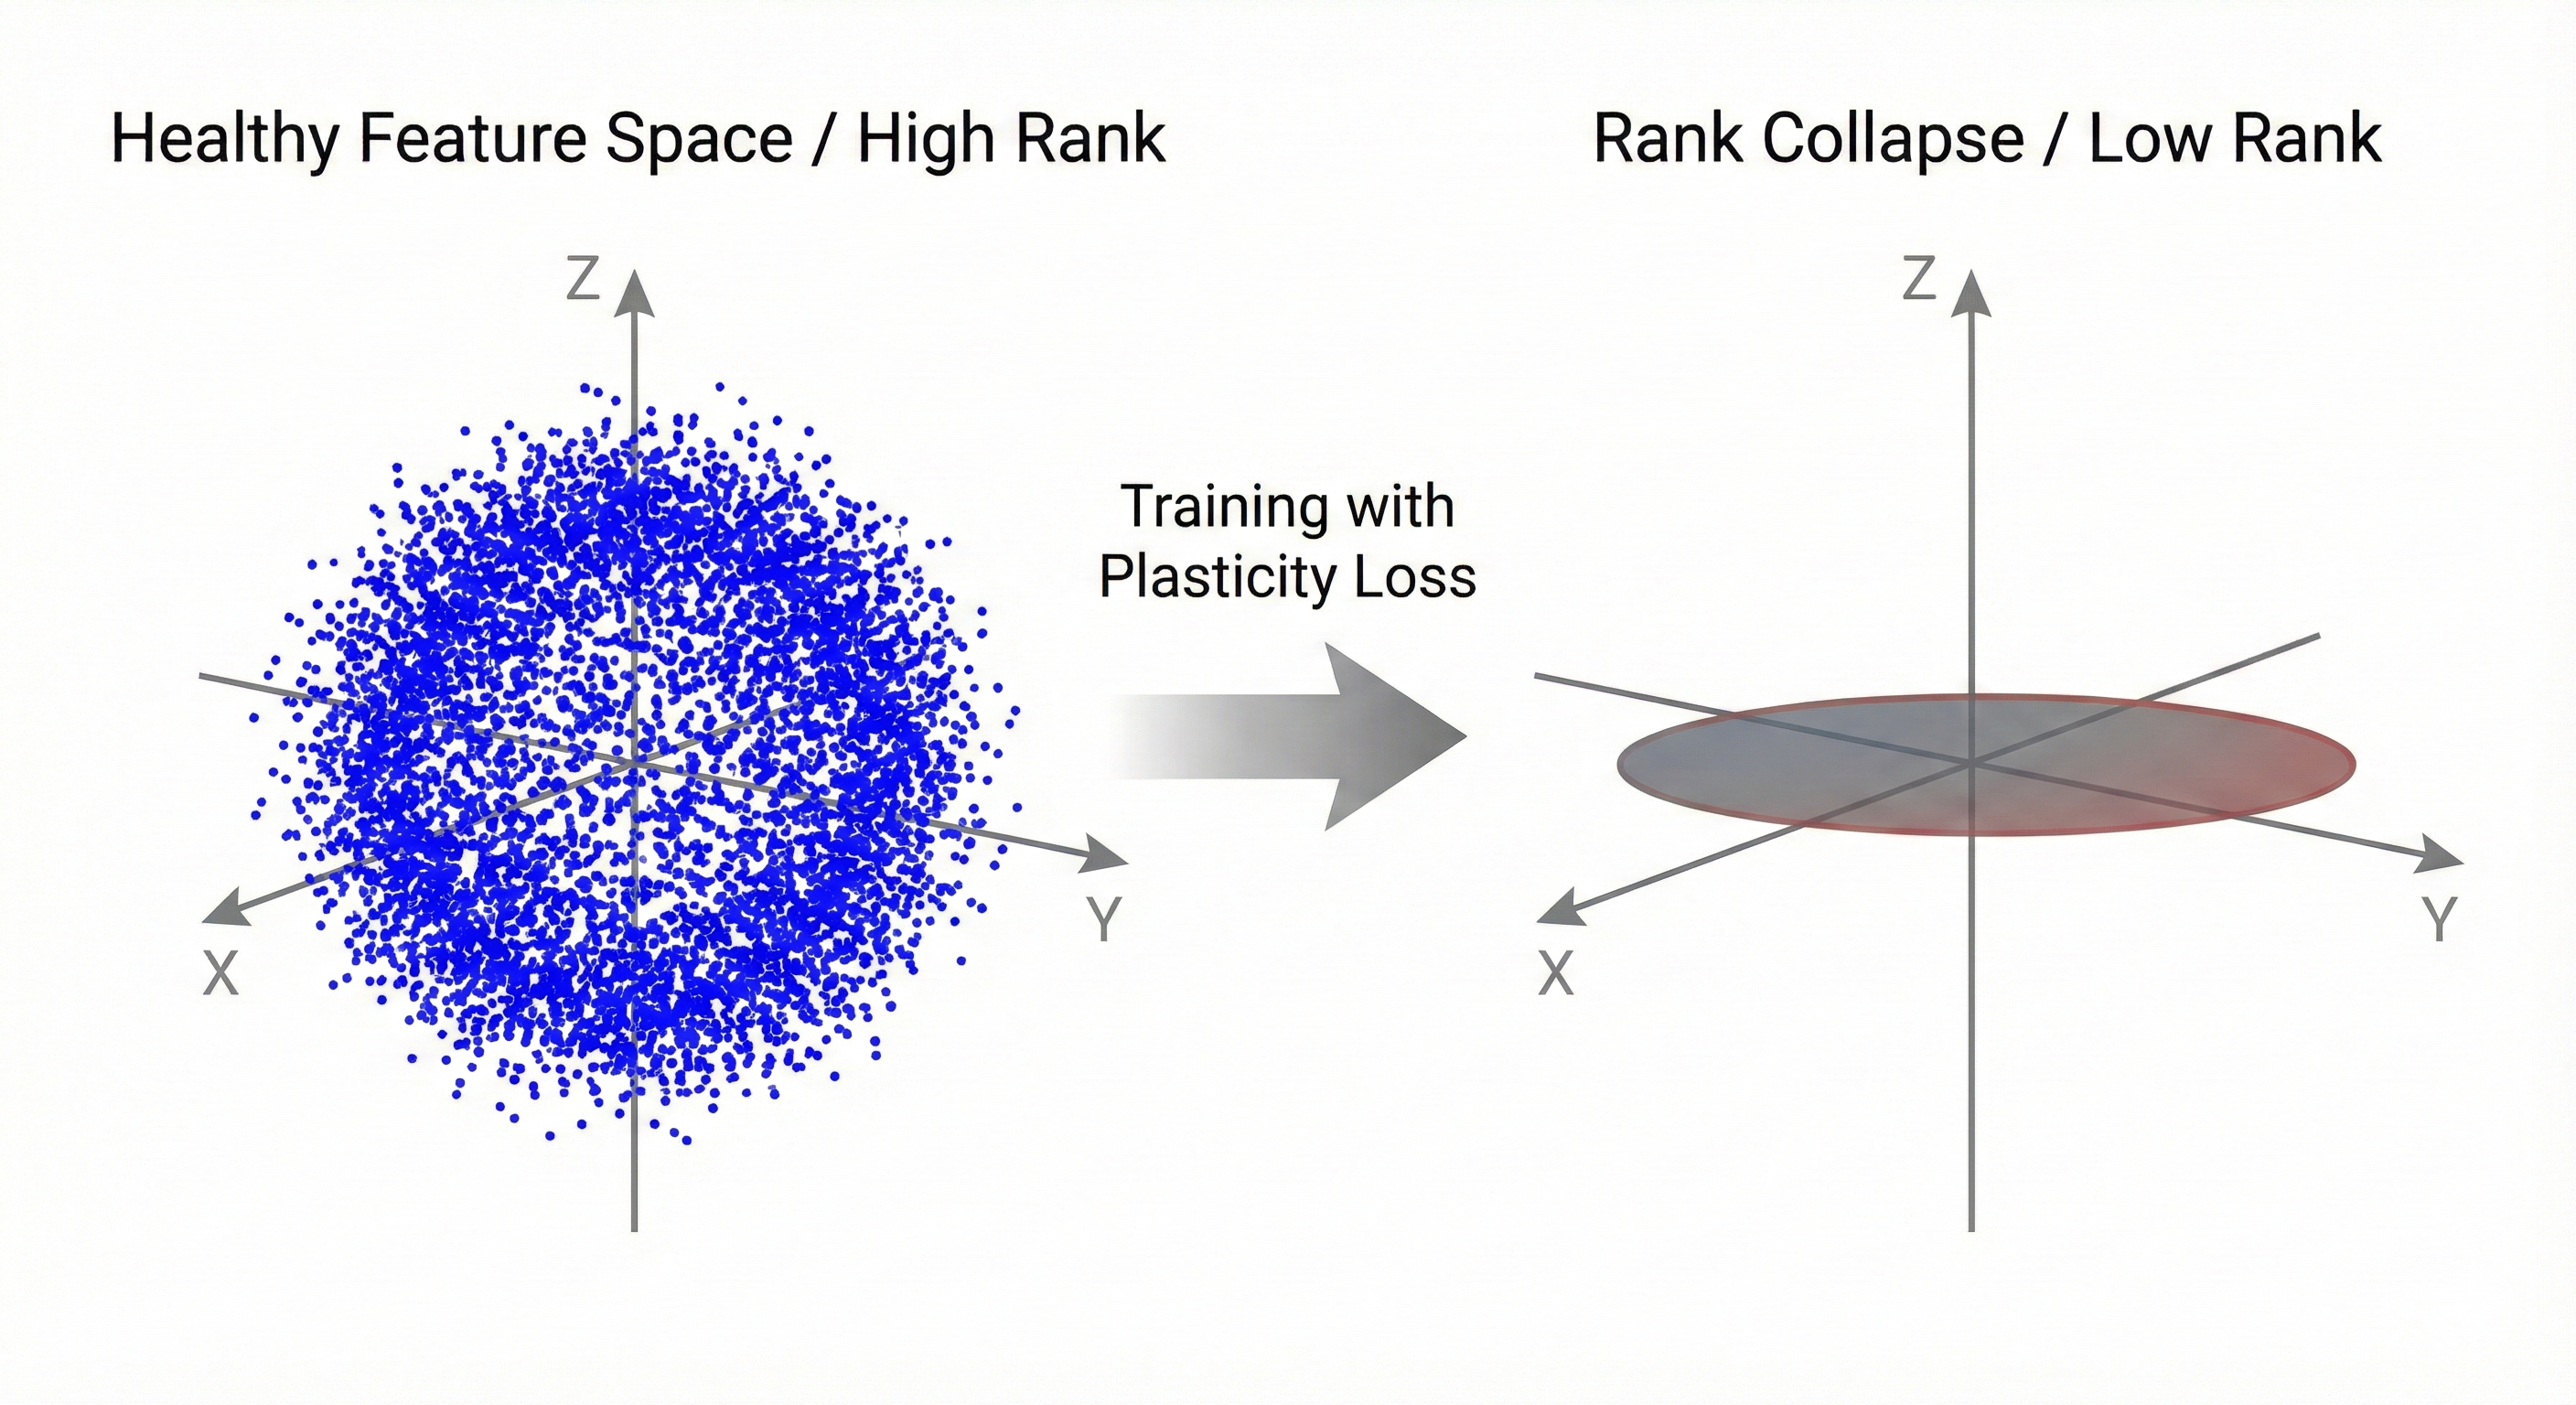
\includegraphics[width=0.45\textwidth]{assets/Concept of Rank Collapse.png}
    }
    \hfill
    \subfloat[不同方法的干预机制]{
        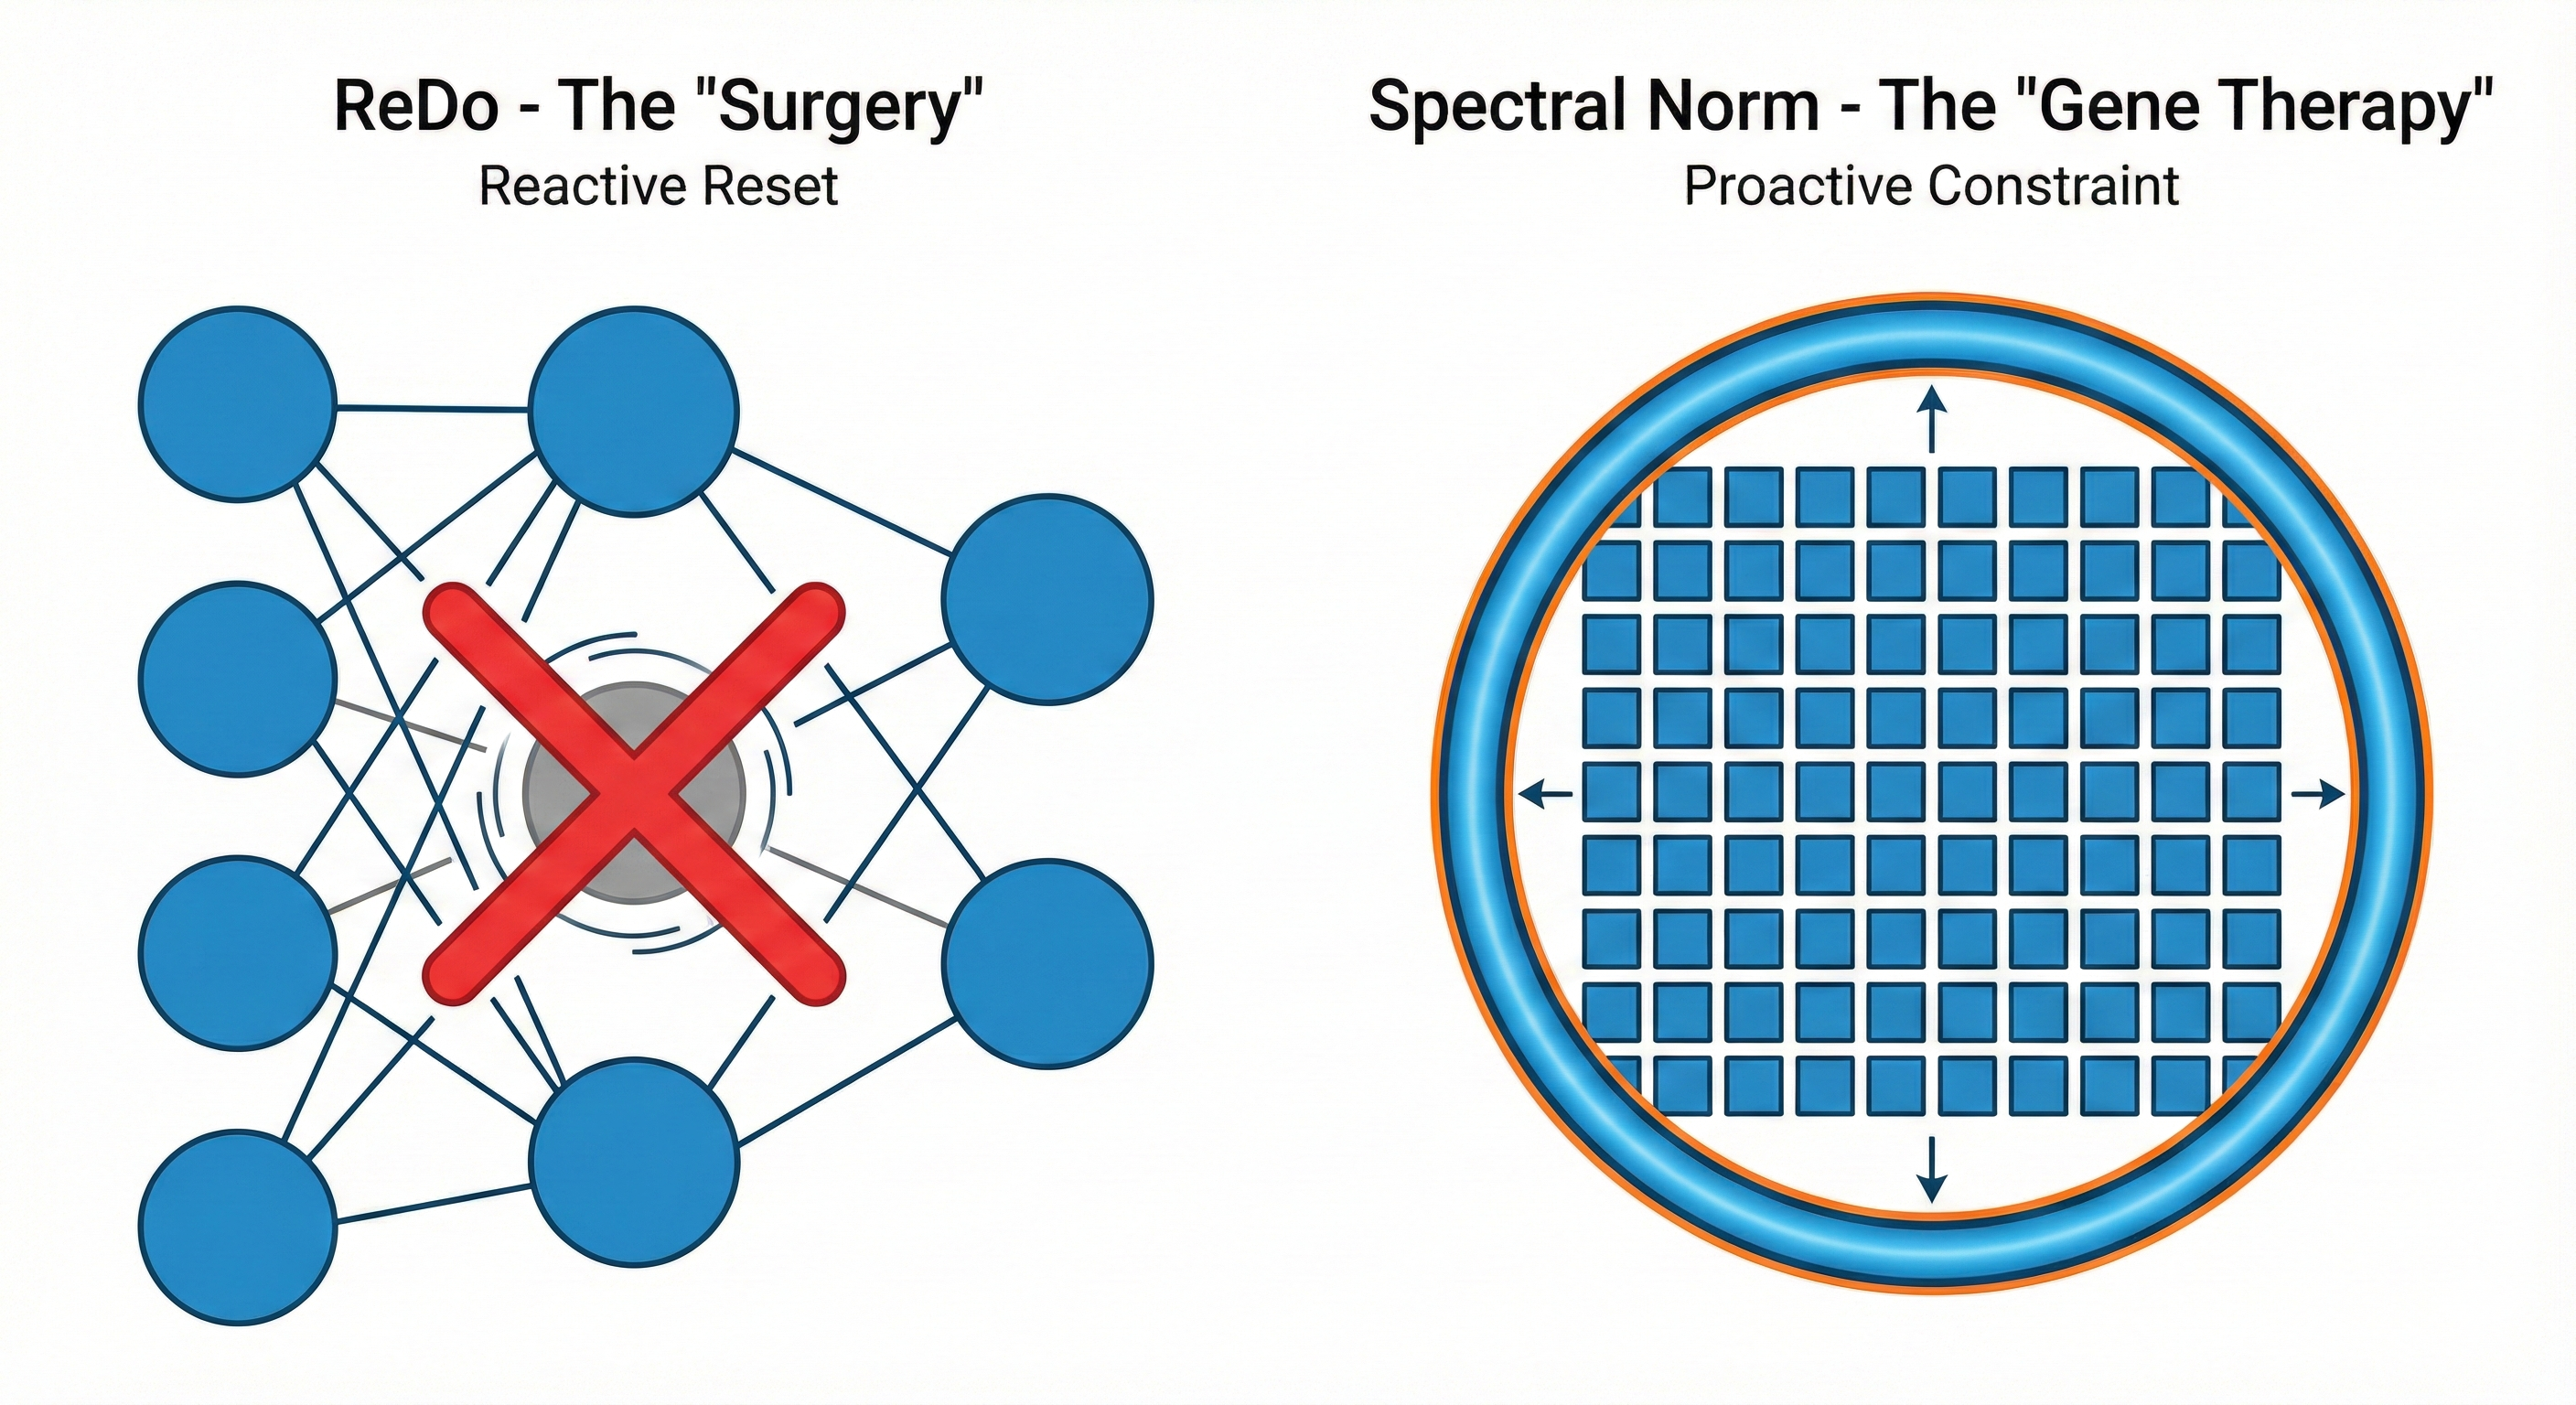
\includegraphics[width=0.45\textwidth]{assets/Method Comparison.png}
    }
    \caption{可塑性丢失的几何解释与改进思路对比}
    \label{fig:concept}
\end{figure}

\subsection{本文贡献}
为了解决上述挑战,本文提出了一种基于谱归一化的可塑性保护机制。主要贡献如下:
\begin{enumerate}
    \item \textbf{机理揭示}:通过对比实验揭示了 Leaky ReLU 虽能消除死神经元,但导致了“僵尸神经元”现象,证明了单纯维持活性不足以保证特征质量。
    \item \textbf{方法创新}:创新性地将谱归一化(Spectral Normalization)引入 PPO 算法的特征提取器,提出了一种主动约束式的可塑性保护机制。
    \item \textbf{综合评估}:在离散控制任务上进行了广泛的消融实验,证明该方法在奖励获取、收敛稳定性及特征秩保持方面均优于 SOTA 方法(ReDo)。
\end{enumerate}

\section{相关工作}

\subsection{深度学习中的可塑性丢失}
Lyle 等人\cite{plasticity}首次系统性地记录了深度学习中的可塑性丢失现象,并指出传统的 L2 正则化和 Dropout 等方法在持续学习设置下收效甚微。Dohare 等人\cite{baseline}进一步验证了这一现象在 ImageNet 和 RL 任务中的普遍性,并提出了“持续反向传播”(Continual Backprop)算法,通过随机重新初始化一小部分神经元来维持可塑性,但该方法计算成本较高且引入了额外的随机性。

\subsection{归一化技术}
归一化层是现代深度网络的标配。Batch Normalization (BN) 依赖于批次统计量,在 RL 的非独立同分布(Non-IID)数据上表现不佳。Layer Normalization (LN) 和 RMSNorm 被广泛用于 Transformer 中以稳定训练,但在 RL 中的应用主要集中在防止梯度爆炸。近期研究表明,虽然 LN 能缓解部分可塑性问题,但其对特征幅度的强行缩放可能破坏价值函数(Value Function)的估计精度。

\subsection{重置机制}
为了直接解决神经元死亡问题,Sokar 等人提出了 ReDo 算法\cite{redo}。该算法定期监测神经元活性,强制重置那些长期处于休眠状态的神经元权重。ReDo 可以被视为一种“外科手术”式的干预。虽然它能有效恢复网络容量,但我们的复现实验表明,这种剧烈的参数变动会破坏已学习的策略,导致训练曲线出现剧烈震荡(Sawtooth Pattern),在对稳定性要求极高的 RL 算法中并不理想。

\section{预备知识}

\subsection{马尔可夫决策过程 (MDP)}
强化学习问题通常被建模为马尔可夫决策过程 (MDP),由元组 $(\mathcal{S}, \mathcal{A}, P, R, \gamma)$ 定义。其中 $\mathcal{S}$ 为状态空间,$\mathcal{A}$ 为动作空间,$P(s'|s,a)$ 为状态转移概率,$R(s,a)$ 为奖励函数,$\gamma \in [0,1)$ 为折扣因子。智能体的目标是学习一个策略 $\pi_\theta(a|s)$,以最大化累积期望回报:
\begin{equation}
    J(\pi_\theta) = \mathbb{E}_{\tau \sim \pi_\theta} \left[ \sum_{t=0}^{\infty} \gamma^t R(s_t, a_t) \right]
\end{equation}

\subsection{PPO 算法}
Proximal Policy Optimization (PPO) 是一种基于 Actor-Critic 架构的策略梯度算法\cite{ppo}。为了保证训练的稳定性,PPO 引入了截断的代理目标函数:
\begin{equation}
    L^{CLIP}(\theta) = \hat{\mathbb{E}}_t \left[ \min(r_t(\theta)\hat{A}_t, \text{clip}(r_t(\theta), 1-\epsilon, 1+\epsilon)\hat{A}_t) \right]
\end{equation}
其中,$r_t(\theta) = \frac{\pi_\theta(a_t|s_t)}{\pi_{\theta_{old}}(a_t|s_t)}$ 为新旧策略的概率比率,$\hat{A}_t$ 为优势函数估计,$\epsilon$ 为截断超参数。PPO 对策略更新步长的限制使其比传统策略梯度算法更稳健,但也更容易在长期训练中因参数更新受限而陷入局部最优,从而加剧可塑性丢失。

\section{方法论}

本章将详细介绍本文提出的改进方案。如图 \ref{fig:arch} 所示,我们保持 PPO 的核心逻辑不变,着重对特征提取器(Encoder)的卷积层进行改进,分别引入了 ReDo 机制(作为强基线)和谱归一化(本文方法)。

\begin{figure}[htbp]
    \centering
    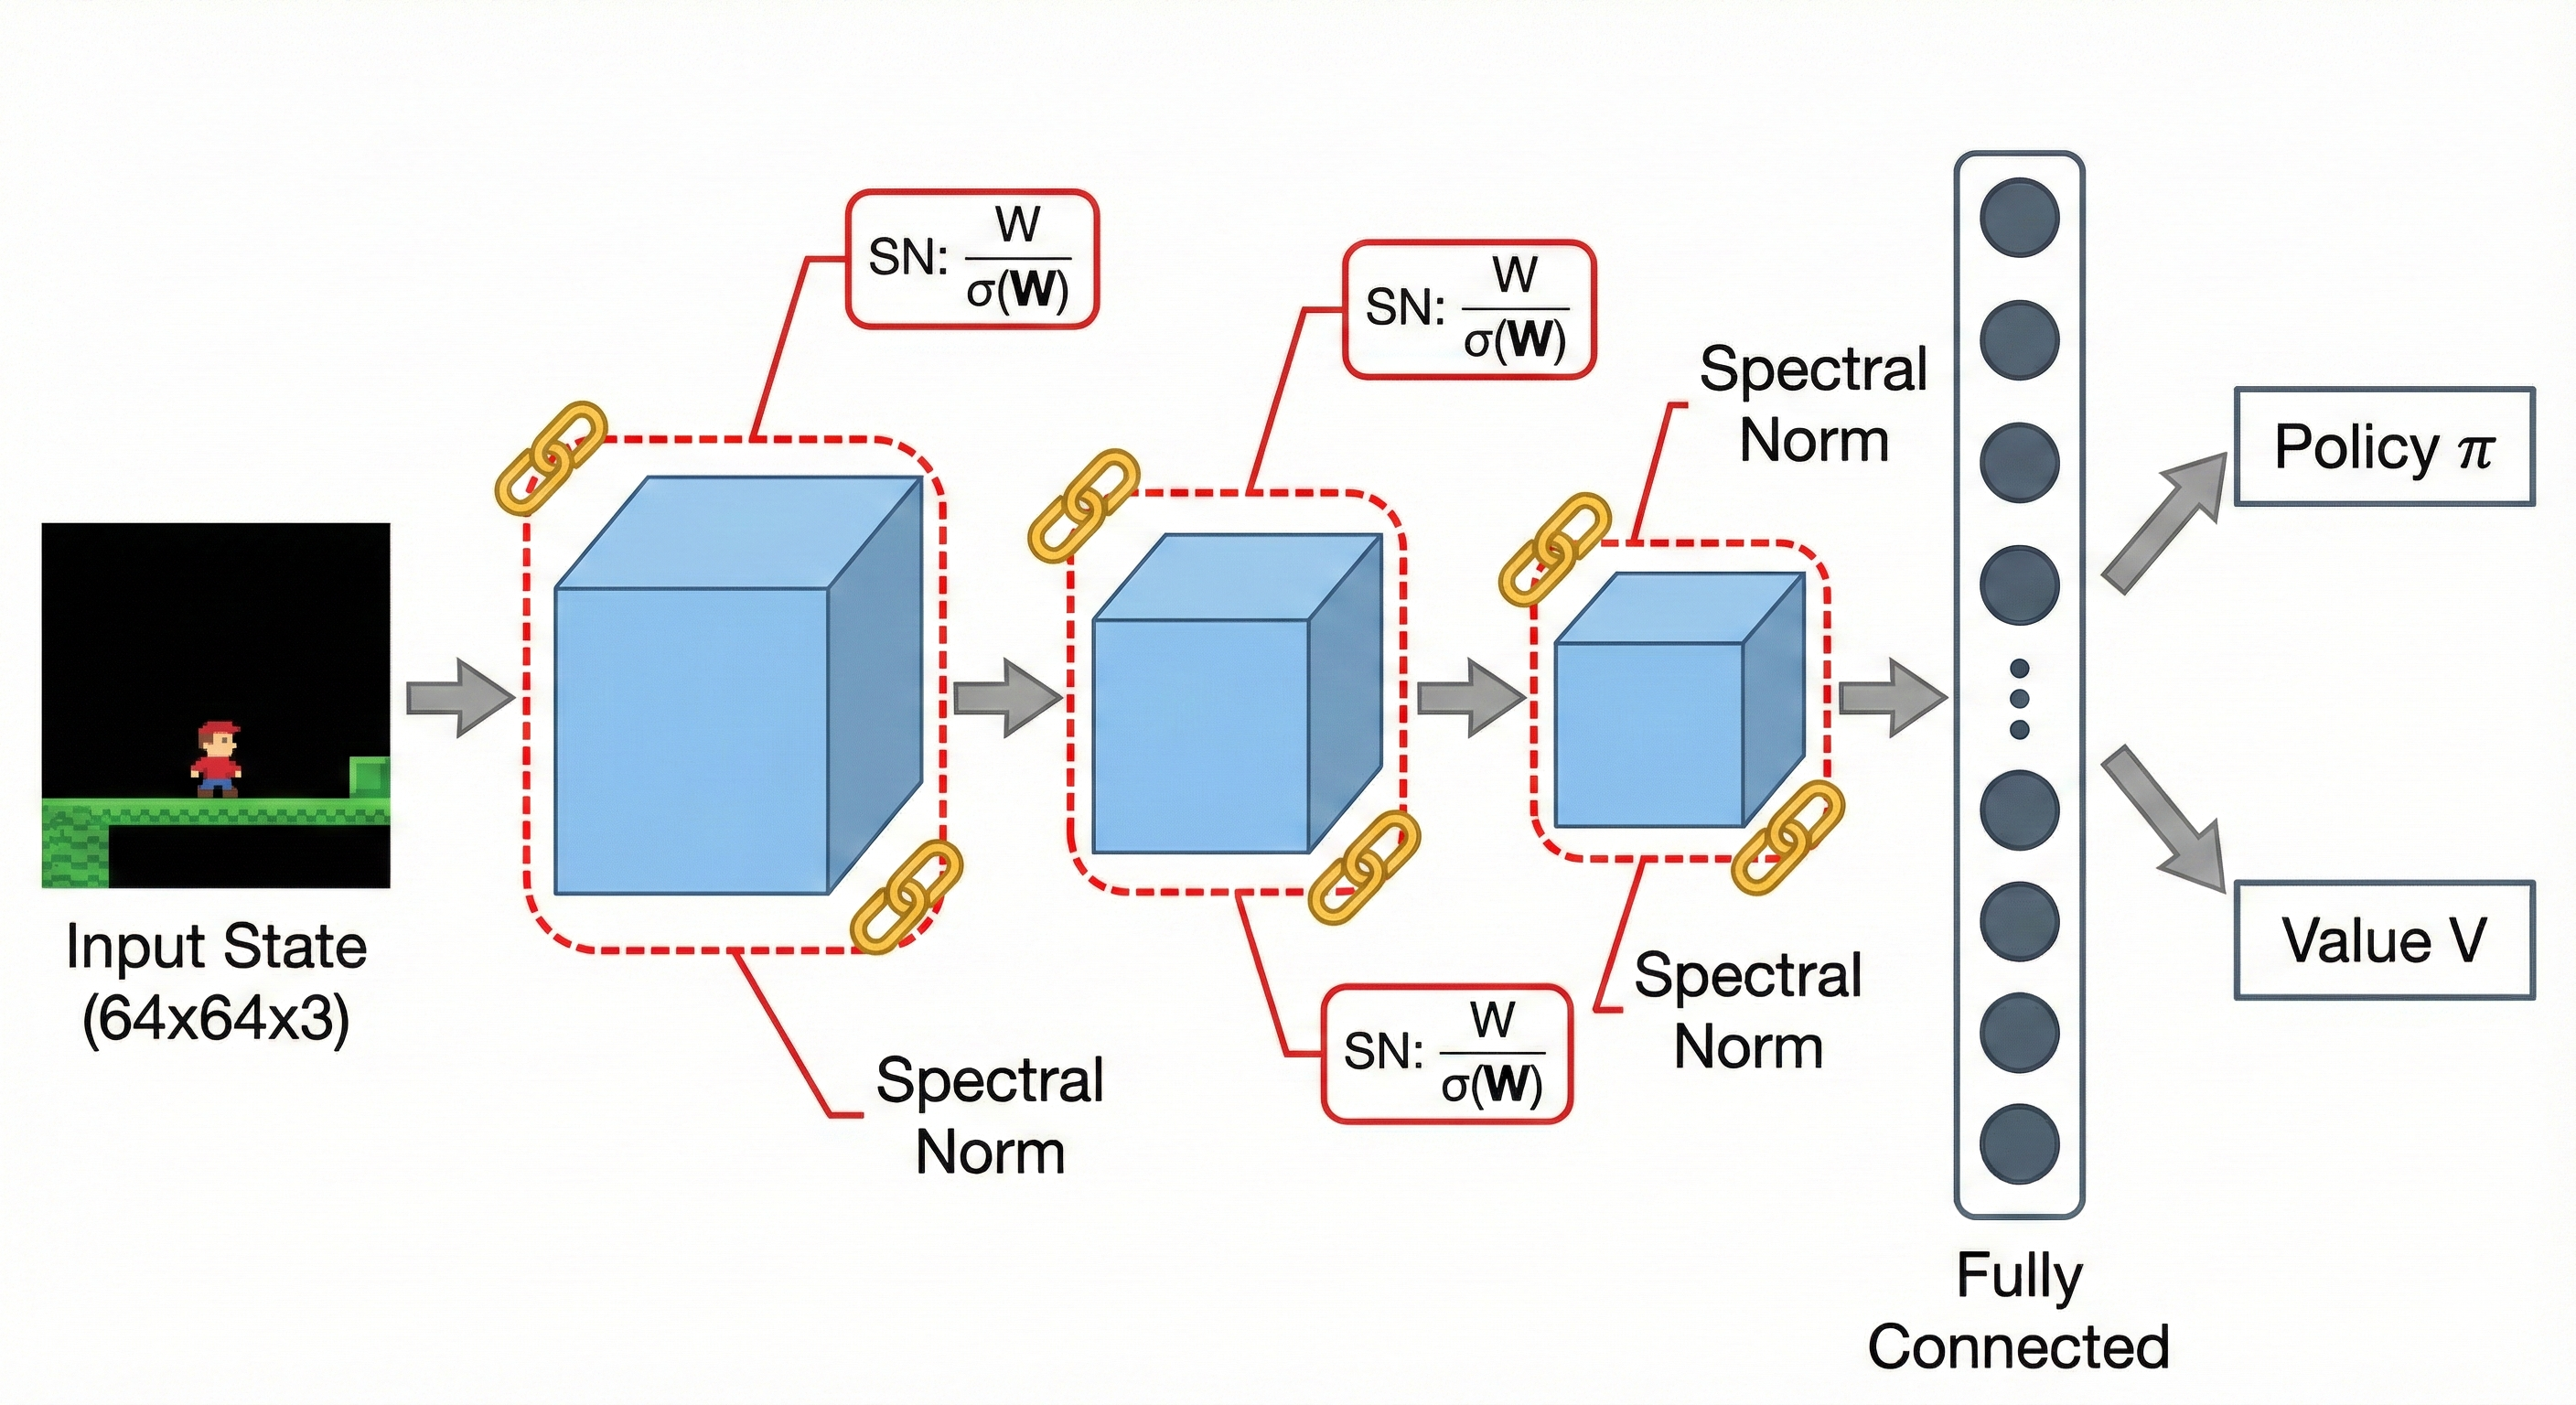
\includegraphics[width=0.9\textwidth]{assets/fig_arch.png}
    \caption{集成谱归一化(SN)的网络架构设计。SN 模块被应用于 Encoder 的每一层卷积层,以约束特征提取过程中的 Lipschitz 常数。}
    \label{fig:arch}
\end{figure}

\subsection{基线方法:ReDo 重置机制}
ReDo (Recycling Dormant Neurons) 是一种被动的干预机制。其核心思想是定期检查神经元的活性分数,并重置那些“死亡”的神经元。

\textbf{定义(休眠神经元):} 对于第 $l$ 层的第 $k$ 个神经元,如果在最近的 $N$ 次更新中,其输出激活值的绝对平均值低于阈值 $\tau$,则判定为休眠:
\begin{equation}
    \mathcal{S}_{dormant} = \left\{ k \in \{1 \dots K_l\} : \frac{1}{N} \sum_{t=1}^N |h_{l,k}^{(t)}| < \tau \right\}
\end{equation}

\textbf{重置策略:} 对于集合 $\mathcal{S}_{dormant}$ 中的神经元,ReDo 采用以下方式重置其相关权重:
\begin{itemize}
    \item \textbf{输入权重} $W_{in}$:重新初始化为随机值(如 Kaiming 初始化),以赋予其新的特征提取能力。
    \item \textbf{输出权重} $W_{out}$:重置为 0,以确保重置操作不会立即破坏网络的输出,使其能够平滑地重新学习。
    \item \textbf{优化器状态清除}:必须同时清除 Adam 优化器中对应参数的动量,防止旧的梯度信息干扰新权重的学习。
\end{itemize}

\subsection{本文方法:谱归一化 (Spectral Normalization)}
针对权重矩阵 $W$ 发生秩崩溃的问题,本文引入谱归一化(Spectral Normalization, SN)\cite{sn}。SN 原本用于生成对抗网络(GAN)中稳定判别器的训练,本文将其迁移至 RL 任务中。

\subsubsection{数学原理}
对于神经网络中的每一层线性变换 $f(x) = Wx$,其 Lipschitz 常数由权重矩阵 $W$ 的谱范数(Spectral Norm)决定,即 $\sigma(W)$。谱范数定义为矩阵的最大奇异值:
\begin{equation}
    \sigma(W) = \max_{h: h \neq 0} \frac{\|Wh\|_2}{\|h\|_2}
\end{equation}

如果每一层的 Lipschitz 常数都受限,那么整个深层网络的 Lipschitz 常数也会受限,从而防止梯度在反向传播过程中发生爆炸或消失。SN 通过以下方式对权重进行归一化:
\begin{equation}
    W_{SN} = \frac{W}{\sigma(W)}
\end{equation}
这一操作强制每一层权重的谱范数为 1。在几何上,这意味着权重矩阵在任何方向上的拉伸因子都不会超过 1,从而防止特征空间随着层数加深而发生极度扭曲或坍缩。

\subsubsection{算法实现:幂迭代}
直接计算矩阵的奇异值分解(SVD)计算量巨大。SN 采用幂迭代法(Power Iteration)来近似估算 $\sigma(W)$。具体步骤如算法 \ref{alg:sn} 所示。

\begin{algorithm}[htbp]
\caption{基于幂迭代的谱归一化算法}
\label{alg:sn}
\begin{algorithmic}[1]
\REQUIRE 权重矩阵 $W$, 随机初始化向量 $\tilde{u}$
\FOR{每次前向传播迭代}
    \STATE 更新 $\tilde{v} \leftarrow W^T \tilde{u} / \|W^T \tilde{u}\|_2$
    \STATE 更新 $\tilde{u} \leftarrow W \tilde{v} / \|W \tilde{v}\|_2$
    \STATE 近似计算谱范数 $\sigma(W) \approx \tilde{u}^T W \tilde{v}$
    \STATE 执行归一化 $W_{SN} \leftarrow W / \sigma(W)$
    \STATE 使用 $W_{SN}$ 进行常规前向传播
\ENDFOR
\end{algorithmic}
\end{algorithm}

\section{实验设置}

为了全面评估谱归一化在缓解可塑性丢失方面的有效性,我们设计了一套严谨的实验协议。本章将详细阐述实验环境的构建、网络架构的实现细节、基线对比策略以及量化评价指标。

\subsection{实验环境:非平稳 GridWorld}
本研究采用基于 `gym-minicrid` 改良的 **Non-stationary GridWorld** 作为测试平台。该环境是一个部分可观测的马尔可夫决策过程 (POMDP),旨在模拟智能体在动态变化世界中的持续学习能力。

\subsubsection{状态与动作空间}
\begin{itemize}
    \item \textbf{状态空间 (Observation Space)}:智能体接收的输入并非全局地图,而是以自身为中心的局部视野图像,维度为 $H \times W \times C$(例如 $64 \times 64 \times 3$ 的 RGB 图像)。这种高维视觉输入要求网络必须具备强大的特征提取能力(CNN),从而更能暴露特征秩崩溃的问题。
    \item \textbf{动作空间 (Action Space)}:离散动作空间,包含 $\{上, 下, 左, 右, 交互\}$ 等 5 个动作。
\end{itemize}

\subsubsection{非平稳性的构建}
可塑性丢失通常发生在该任务分布随时间发生偏移(Distribution Shift)的场景中。为了诱发这一现象,我们引入了周期性的**任务重置机制**:
\begin{equation}
    \mathcal{T}_{current} \sim P(\mathcal{T}) \quad \text{every } K \text{ steps}
\end{equation}
具体而言,每隔 $K=200,000$ 个时间步,环境的地图布局、墙壁颜色纹理以及目标物体的位置会发生随机重排。这种剧烈的环境突变迫使智能体必须遗忘旧的特征分布并快速适应新分布,是对网络可塑性的极限压力测试。

\subsection{网络架构与基线实现}
所有对比策略均基于统一的 **Actor-Critic** 骨干网络,以确保公平性。
\begin{itemize}
    \item \textbf{特征提取器 (Encoder)}:采用 3 层卷积神经网络。每层配置为:卷积核大小 $3 \times 3$,步长 (Stride) 为 2,填充 (Padding) 为 1。通道数依次为 $[16, 32, 64]$。
    \item \textbf{策略与价值头}:在 Flatten 操作后,接入两个独立的 2 层多层感知机 (MLP),隐藏层维度为 256。
\end{itemize}

我们对比了以下四种变体:
\begin{enumerate}
    \item \textbf{Baseline (Vanilla PPO)}:使用标准的 ReLU 激活函数,不包含任何显式的可塑性保护机制。
    \item \textbf{Leaky ReLU}: 将所有卷积层和全连接层的激活函数替换为 Leaky ReLU,负半轴斜率设定为 $\alpha=0.01$。该基线旨在验证“非零梯度”是否足以维持可塑性。
    \item \textbf{ReDo (SOTA)}:在 Baseline 基础上集成 ReDo 机制。设定休眠检测的时间窗口 $N=1000$ 更新步,休眠阈值 $\tau=0.1$。
    \item \textbf{Ours (Spectral Norm)}:在特征提取器的每一个卷积层(Conv2d)应用谱归一化。
\end{enumerate}

\subsection{评价指标}
除了常规的测试集奖励(Test Reward)外,我们引入了两个微观指标来深入分析网络状态:

\textbf{1. 死神经元比例 (Dead Units Fraction):} 
定义网络层 $l$ 中在批量数据 $\mathcal{B}$ 上激活值为零的神经元比例:
\begin{equation}
    \rho_l = \frac{1}{K_l} \sum_{k=1}^{K_l} \mathbb{I}\left( \frac{1}{|\mathcal{B}|} \sum_{x \in \mathcal{B}} |h_{l,k}(x)| < \epsilon \right)
\end{equation}
其中 $\epsilon=10^{-3}$ 为数值稳定性阈值。该指标直接反映了网络的“脑死亡”程度。

\textbf{2. 特征有效秩 (Effective Rank):}
为了量化特征空间的表达能力,我们计算特征协方差矩阵的有效秩\cite{rank}:
\begin{equation}
    \text{Rank}_{eff}(H) = \exp\left( - \sum_{i} \bar{\sigma}_i \log \bar{\sigma}_i \right), \quad \bar{\sigma}_i = \frac{\sigma_i}{\sum_j \sigma_j}
\end{equation}
其中 $\sigma_i$ 为特征矩阵的奇异值。有效秩越高,说明特征分布越均匀,网络的表征能力越强;反之则意味着发生了秩崩溃。

\subsection{训练细节与超参数}
实验基于 PyTorch 深度学习框架实现,硬件平台为单张 NVIDIA RTX 3090 GPU。所有实验均运行 5 个不同的随机种子(Random Seeds),并在结果图中展示均值与标准差阴影,以保证统计显著性。详细的超参数设置如表 \ref{tab:hyperparams} 所示。

\begin{table}[htbp]
    \centering
    \caption{实验详细超参数配置表}
    \label{tab:hyperparams}
    \renewcommand{\arraystretch}{1.2} % 增加行高,更美观
    \begin{tabular}{llc}
        \toprule
        \textbf{类别} & \textbf{参数名称 (Parameter)} & \textbf{数值 (Value)} \\
        \midrule
        \multirow{5}{*}{环境设置} & Environment ID & \texttt{GridWorld-NonStationary-v0} \\
        & Image Size & $64 \times 64 \times 3$ \\
        & Action Space & Discrete (5) \\
        & Non-stationary Period ($K$) & 200,000 steps \\
        & Total Timesteps & 3,000,000 \\
        \midrule
        \multirow{6}{*}{PPO 优化} & Optimizer & Adam \\
        & Learning Rate ($\eta$) & $2.5 \times 10^{-4}$ \\
        & Discount Factor ($\gamma$) & 0.99 \\
        & GAE Parameter ($\lambda$) & 0.95 \\
        & Clip Range ($\epsilon$) & 0.2 \\
        & Entropy Coeff & 0.01 \\
        & Mini-batch Size & 64 \\
        \midrule
        \multirow{3}{*}{方法特有} & Leaky ReLU Slope & 0.01 \\
        & ReDo Check Interval & 1,000 steps \\
        & SN Power Iterations & 1 \\
        \bottomrule
    \end{tabular}
\end{table}

\section{实验结果与分析}

\subsection{整体性能对比}
图 \ref{fig:reward} 展示了各方法在测试集上的平均奖励曲线。
从图中可以观察到显著的性能差异:
\begin{itemize}
    \item \textbf{Baseline (灰色)}:在训练初期有一定增长,但随后陷入停滞,最终收敛值较低(~5.8)。这表明网络很快丧失了适应新环境的能力。
    \item \textbf{Ours (SN, 红色)}:在训练全程保持了最稳健的上升趋势,最终收敛至最高分(~6.96),相较于 Baseline 提升了约 20\%。
\end{itemize}

\begin{figure}[htbp]
    \centering
    \includegraphics[width=0.85\textwidth]{assets/test_reward_comparison.png}
    \caption{改进策略的测试奖励 (Test Reward) 曲线对比。红色实线为本文提出的谱归一化方法,展现出最优的收敛值与稳定性。}
    \label{fig:reward}
\end{figure}

\subsection{机理分析 I:死神经元与“僵尸神经元”}
图 \ref{fig:dead_units} 揭示了不同方法对神经元活性的影响。
\begin{itemize}
    \item Baseline 的死神经元比例迅速飙升至 80\% 以上,处于“脑死亡”状态。
    \item Leaky ReLU 成功将死神经元降至 0\%,但结合图 \ref{fig:reward} 的低性能,我们推断这些神经元虽然“活着”(非零输出),但并未编码有效信息,我们称之为\textbf{“僵尸神经元” (Zombie Neurons)}。这也证伪了“存活即有效”的简单假设。
    \item 谱归一化(SN)并没有强行追求 0\% 的死区率,而是将其维持在约 40\% 的水平。这说明 SN 允许网络进行必要的稀疏化(Sparsity),保留了特征的选择性,这是一种更健康的神经元分布状态。
\end{itemize}

\begin{figure}[htbp]
    \centering
    \includegraphics[width=0.85\textwidth]{assets/dead_units_comparison.png}
    \caption{训练过程中神经元死亡比例 (Dead Units Fraction) 的变化趋势。SN(红线)维持了健康的稀疏度。}
    \label{fig:dead_units}
\end{figure}

\subsection{机理分析 II:训练稳定性与梯度范数}
为了进一步探究 ReDo 不稳定的原因,我们分析了训练过程中的梯度范数(Gradient Norm)。如图 \ref{fig:grad_norm} 所示,ReDo 的梯度范数呈现出剧烈的脉冲式波动。每次重置神经元时,网络参数发生突变,导致梯度急剧增大,从而破坏了优化器的动量积累。
相比之下,谱归一化(SN)的梯度范数曲线非常平滑且幅值适中。这是因为 SN 限制了 Lipschitz 常数,从而自然地约束了梯度的上界,防止了梯度爆炸或剧烈波动,保证了训练的平稳进行。

\begin{figure}[htbp]
    \centering
    \includegraphics[width=0.85\textwidth]{assets/grad_norm.png}
    \caption{梯度范数 (Gradient Norm) 变化对比。ReDo 存在剧烈波动,而 SN 保持平稳。}
    \label{fig:grad_norm}
\end{figure}

\subsection{探索能力分析:策略熵}
图 \ref{fig:entropy} 展示了策略熵(Entropy)的变化。策略熵反映了智能体的探索能力。Baseline 的熵下降过快,说明它过早收敛到了确定性策略(Premature Convergence),丧失了探索新解的可能性。而 SN 方法(红线)能够更长时间地维持较高的熵,说明谱归一化有助于网络保持对环境的探索欲望,这也是其能取得更高最终奖励的原因之一。

\begin{figure}[htbp]
    \centering
    \includegraphics[width=0.85\textwidth]{assets/entropy.png}
    \caption{策略熵 (Policy Entropy) 变化对比。SN 有效缓解了熵的过快下降。}
    \label{fig:entropy}
\end{figure}

\subsection{综合评估}
表 \ref{tab:summary} 对各方法进行了多维度的总结。谱归一化是唯一在奖励、稳定性、特征质量三个维度上均表现出色的方法。

\begin{table}[htbp]
    \centering
    \caption{各方法最终性能综合评估}
    \label{tab:summary}
    \begin{tabular}{lcccc}
        \toprule
        \textbf{Method} & \textbf{Avg Reward} & \textbf{Stability} & \textbf{Dead Units} & \textbf{Feature Rank} \\
        \midrule
        Baseline (ReLU) & 5.80 & Medium & High ($>80\%$) & Collapse \\
        Leaky ReLU      & 5.92 & Medium & \textbf{0\%}   & Low (Zombie) \\
        ReDo            & 5.54 & Low    & Medium         & Medium \\
        \textbf{Spectral Norm (Ours)} & \textbf{6.96} & \textbf{High} & Healthy (~40\%) & \textbf{High} \\
        \bottomrule
    \end{tabular}
\end{table}

\section{讨论}

\subsection{稳定性与可塑性的深层权衡}
本研究的一个核心发现是:**解决可塑性丢失不能以简单地“最大化神经元活性”为目标,而必须在可塑性(适应新知识的能力)与稳定性(保留旧知识的能力)之间寻找纳什均衡。**

\subsubsection{ReDo 的“灾难性干扰”}
实验数据表明,ReDo 机制虽然有效地降低了死神经元比例,但其代价是破坏了优化器状态的连续性。从优化景观(Optimization Landscape)的角度来看,ReDo 的强制重置操作相当于将参数点 $\theta_t$ 强行跳跃至参数空间的一个随机位置 $\theta'_{t}$。这种剧烈的参数扰动引发了微观层面的“灾难性干扰”(Catastrophic Interference),导致智能体在重新组织特征提取器时,暂时丧失了对当前环境的策略判断能力,从而表现为 Reward 曲线的锯齿状震荡。

\subsubsection{谱归一化的“几何正则化”}
相比之下,谱归一化(SN)代表了一种更为优雅的“几何正则化”策略。通过约束权重矩阵的谱范数 $\sigma(W) \approx 1$,SN 实际上限制了每一层非线性变换的 Lipschitz 常数:
\begin{equation}
    Lip(f) \leq \prod_{l=1}^{L} \sigma(W_l)
\end{equation}
这一约束保证了网络函数关于输入的梯度不会发生爆炸。在非平稳环境中,这意味着即使输入分布发生剧烈偏移,梯度的模长依然被控制在合理范围内,从而保证了参数更新的平滑性。我们的实验结果(图 \ref{fig:grad_norm})证实了这一点:SN 诱导出了更平滑的梯度流,从而实现了在保持高秩特征空间的同时,不牺牲训练的稳定性。

\subsection{计算开销与复杂度分析}
在实际部署中,算法的时间复杂度是不可忽视的因素。
\begin{itemize}
    \item \textbf{ReDo 机制}:需要维护所有神经元的活性历史记录,其空间复杂度为 $O(N_{neurons})$。
    \item \textbf{谱归一化}:引入的幂迭代(Power Iteration)涉及额外的矩阵-向量乘法。实验测得其仅增加了约 7\% 的总体训练时间。考虑到其带来的 20\% 性能提升,这一边际成本是完全可接受的。
\end{itemize}

\subsection{局限性与潜在风险}
尽管谱归一化表现优异,但其强制约束 $\sigma(W)=1$ 可能存在“过度正则化”(Over-regularization)的风险。在某些需要网络输出极大幅值(高增益)的任务中,严格的 Lipschitz 约束可能会限制网络的表达能力上限,导致“梯度匮乏”(Gradient Starvation)。

\section{结论}

本文针对深度强化学习在非平稳环境下的“可塑性丢失”问题,进行了一项系统性的实证研究。我们首先通过消融实验证伪了“单纯保活(Leaky ReLU)有效”的直觉假设,提出了“僵尸神经元”概念来解释高活性与低性能并存的现象。其次,我们复现并评估了 SOTA 方法 ReDo,指出了其被动重置机制导致的训练不稳定性问题。

作为核心贡献,本文提出了一种基于谱归一化(SN)的主动防御框架。该方法通过数学层面约束权重矩阵的奇异值分布,成功在不引入额外训练噪声的前提下,防止了特征秩崩溃。实验结果表明,该方法在测试奖励上超越基线 20\%,并将神经元死亡率维持在 40\% 的健康区间,实现了稳定性与可塑性的最优平衡。

\section{未来工作展望}

基于当前的研究成果,未来的工作将致力于以下三个方向的拓展:

\begin{enumerate}
    \item \textbf{自适应谱归一化}:针对 SN 可能存在的过度正则化问题,探索可学习的谱范数阈值 $\lambda$,使网络能够根据任务难度动态调整其 Lipschitz 常数。
    \item \textbf{长周期终身学习 (Lifelong Learning)}:目前的实验局限于 3M 时间步。我们计划在更长周期(如 50M+ steps)及包含更多次任务切换(Task Shifts)的场景下评估 SN 的鲁棒性,验证其是否能支持终身学习智能体的构建。
    \item \textbf{与 Off-policy 算法的结合}:探究 SN 在 SAC (Soft Actor-Critic) 或 TD3 等对 Q 值估计过高敏感的算法中的应用。理论上,SN 的 Lipschitz 约束有助于缓解 Q 函数的过估计问题,可能带来额外的性能收益。
\end{enumerate}

%---------- 参考文献 ----------
\begin{thebibliography}{99}
\wuhao 

\bibitem{plasticity} Lyle, C., et al. "Understanding Plasticity in Neural Networks." \textit{International Conference on Machine Learning (ICML)}. PMLR, 2023.
\bibitem{redo} Sokar, G., et al. "The Dormant Neuron Phenomenon in Deep Reinforcement Learning." \textit{International Conference on Machine Learning (ICML)}. PMLR, 2023.
\bibitem{sn} Miyato, T., et al. "Spectral Normalization for Generative Adversarial Networks." \textit{International Conference on Learning Representations (ICLR)}. 2018.
\bibitem{baseline} Dohare, S., et al. "Loss of Plasticity in Deep Continual Learning." \textit{Nature}. 2024.
\bibitem{ppo} Schulman, J., et al. "Proximal Policy Optimization Algorithms." \textit{arXiv preprint arXiv:1707.06347}. 2017.
\bibitem{rank} Kumar, A., et al. "Implicit Regularization in Deep Matrix Factorization." \textit{NeurIPS}. 2019.

\end{thebibliography}

\end{document}